\documentclass[a4paper, 12pt]{article}

%\usepackage{cmap}
\usepackage[T2A]{fontenc}
\usepackage[utf8]{inputenc}
\usepackage[english, russian]{babel}
\usepackage{graphicx}
\usepackage[top=1in, bottom=1in, left=3.2cm, right=2.6cm]{geometry}
\graphicspath{./}
\usepackage{biblatex}
\addbibresource{lib.bib}
\linespread{1.5}
\usepackage{ragged2e}
\justifying
\usepackage{listings}
\usepackage{color}
\usepackage{amsmath}


\begin{document}
	
\begin{titlepage}
	\fontsize{12pt}{12pt}\selectfont
	\begin{figure}[t!]
		\centering
		
\includegraphics[scale=0.8]{bmstu}
	\end{figure}
	
	\noindent\rule{15cm}{3pt}
	\newline\newline
	\noindent 
	ФАКУЛЬТЕТ 
	\underline{«Информатика и системы управления»} \newline
	
	\noindent КАФЕДРА \underline{«Программное обеспечение ЭВМ и информационные технологии»}\newline\newline\newline\newline\newline
	
	\centering {\Large \textbf{Отчет по лабораторной работе № 2}}
	\vspace{4mm}
	
	\centering {\Large \textbf{По курсу:} Моделирование
		\vspace{8mm}}
	\\ \centering {\Large \textbf{На тему:} Цепи Маркова}
	\vspace{20mm}
	
	
	\begin{flushright}
		{\small	\textbf{Студент:}\\Андреев Александр Алексеевич \\ \textbf{Группа:} ИУ7-74Б
			\vspace{3mm}
			\\\textbf{Преподователь:} \\ Рудаков Игорь Владимирович }
	\end{flushright}
	
	\begin{center}
		\vfill
		Москва, \the\year
		~г.
	\end{center}
\end{titlepage}

\tableofcontents
\clearpage
\newpage


\section{{Задание}}

\hspace*{5mm} Для сложной системы S, имеющей не более 10 состояний, необходимо определить время пребывания сложной системы в каждом из состояний. На вход подается матрица, на пересечении строк и столбцов которой находятся интенсивности переходов.

\section{{Теоритическая часть}}
Случайный процесс называется Марковским, если он обладает следующим свойством: для каждого момента времени $t_0$ вероятность любого состояния системы в будущем $t > t_0$ зависит только от ее состояния в настоящем, то есть при $t = t_0$, и не зависит от того когда и каким образом система пришла в это состояние. Не зависит от того, как процесс развивался в прошлом. В природе нет таких процессов, но существует ряд процессов, которые могут некоторыми методами быть сведены к Марковским процессам. Для Марковских процессов хорошо работают Уравнения Колмагорова.

По модели из условия строятся уравнения Колмогорова: в левой части уравнений находится производная вероятности состояний, а правая часть содержит члены по количеству переходов, связанных с текущим состоянием. Если направление перехода в текущее состояние, то соответствующий член имеет знак минус, если направление из состояния, то плюс. Каждый член равен произведению плотности вероятности перехода на вероятость того состояния, из которого идет этот переход.

Поскольку модель имеет установившийся режим, то левые части уравненя будут равно нулю. Далее вводится уравнение нормировки и производится подсчет.

Получившиеся вероятности являются средним относительным временем пребывания системы в данном состоянии.

Среднее время находится по формуле \ref{eq:time}

\begin{equation}\label{eq:time}
	t_i = \frac{1 - p_i}{p_i \cdot \sum_{i \ne j}\lambda_{ij}}
\end{equation}


\section{{Результаты}}
\begin{figure}[h!]
	\centering 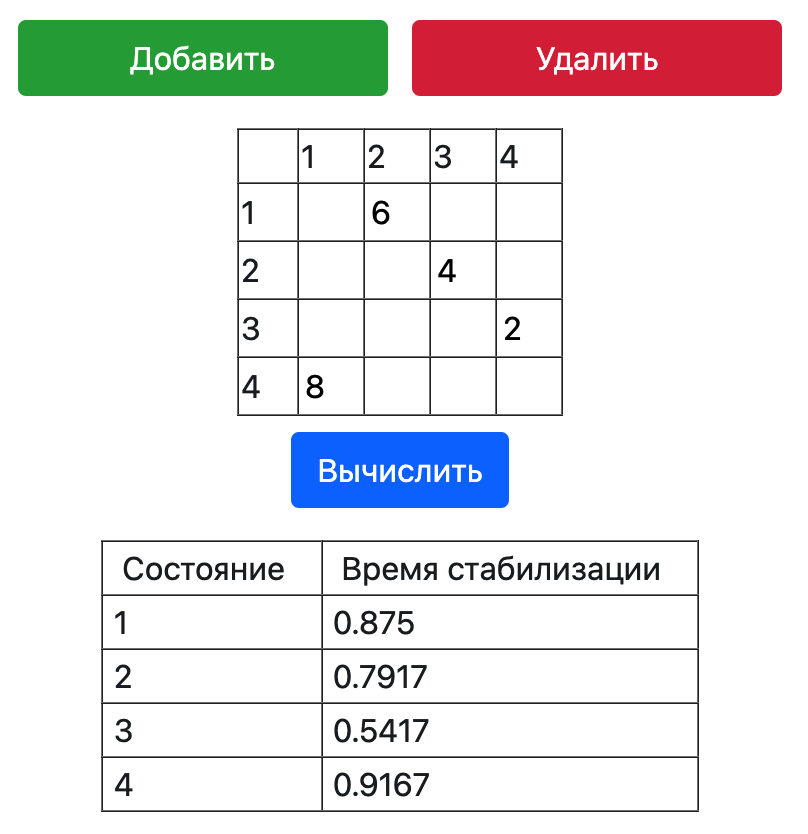
\includegraphics[scale=0.6]{1}
	\centering\caption{Пример работы для 4 cостояний}
\end{figure}
\begin{figure}[h!]
	\centering 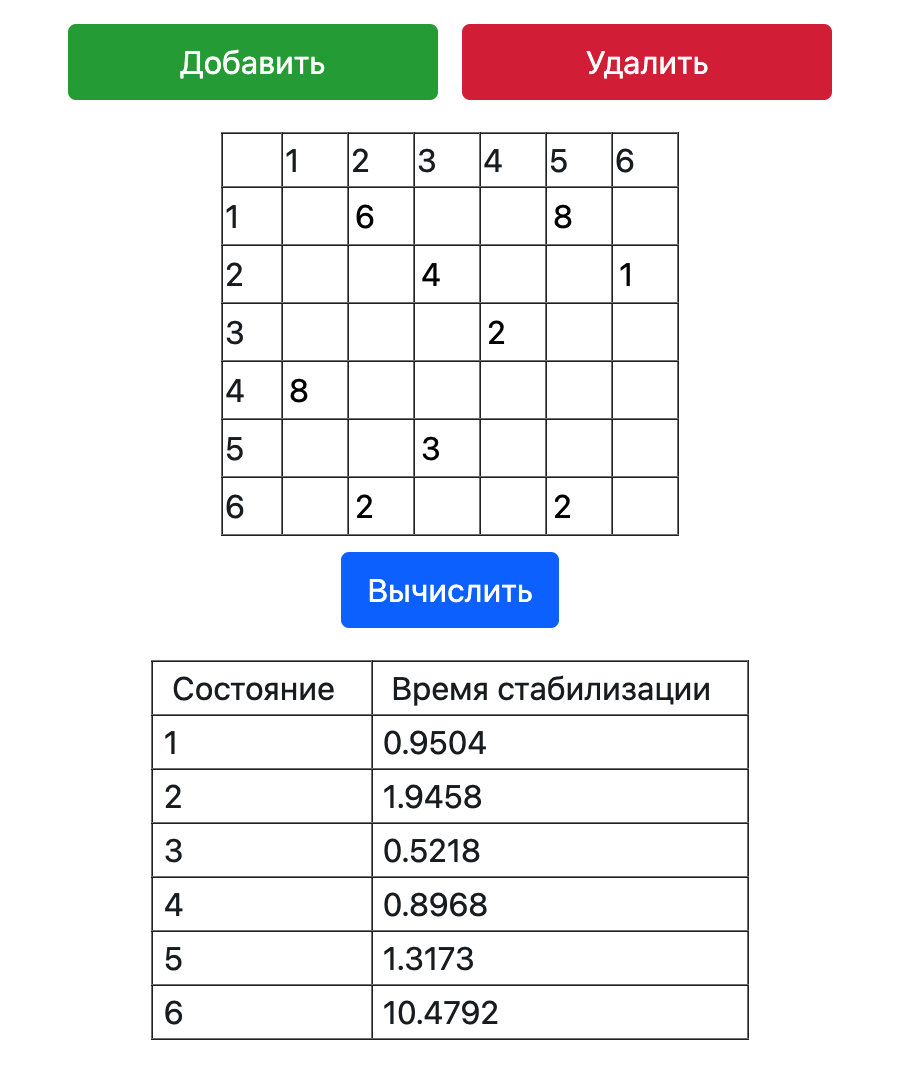
\includegraphics[scale=0.6]{2}
	\centering\caption{Пример работы для 6 состояний}
\end{figure}
\clearpage
\newpage
\begin{figure}[h!]
	\centering 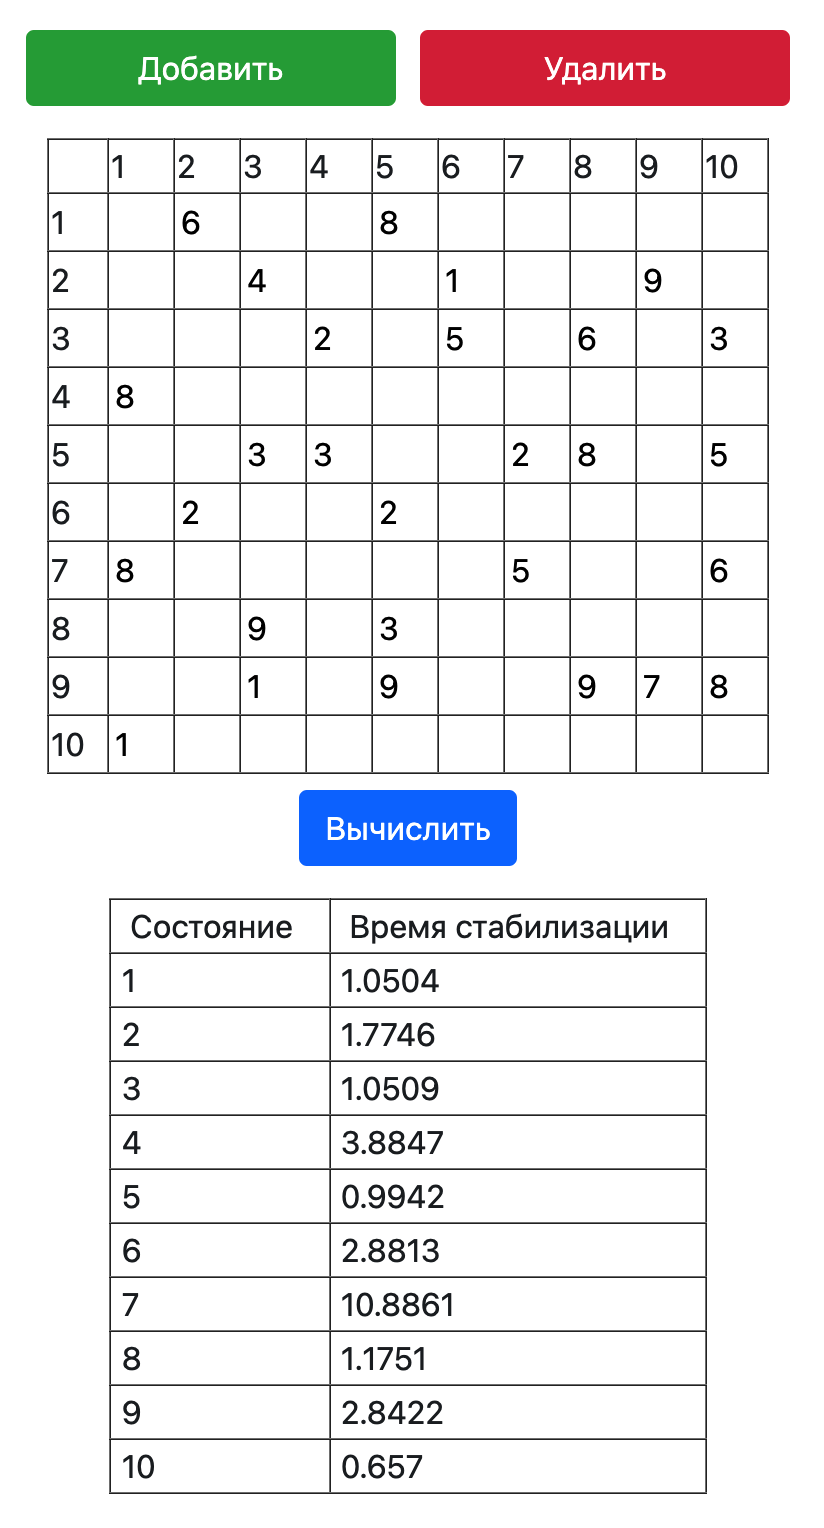
\includegraphics[scale=0.6]{3}
	\centering\caption{Пример работы для 10 состояний}
\end{figure}
\clearpage
\newpage
\section{Листинг кода}
\definecolor{codegreen}{rgb}{0,0.6,0}
\definecolor{codegray}{rgb}{0.5,0.5,0.5}
\definecolor{codepurple}{rgb}{0.58,0,0.82}
\definecolor{backcolour}{rgb}{0.95,0.95,0.92}

\lstdefinestyle{mystyle}{
	backgroundcolor=\color{backcolour},   
	commentstyle=\color{codegreen},
	keywordstyle=\color{magenta},
	numberstyle=\tiny\color{codegray},
	stringstyle=\color{codepurple},
	basicstyle=\ttfamily\footnotesize,
	breakatwhitespace=false,         
	breaklines=false,                 
	captionpos=b,                    
	keepspaces=true,                 
	numbers=left,                    
	numbersep=5pt,                  
	showspaces=false,                
	showstringspaces=false,
	showtabs=false,                  
	tabsize=4
}

\lstset{style=mystyle}

\begin{lstlisting}[language=Python, caption = Программная реализация определения времени пребывания сложной системы в каждом из состояний]
# Created by Andreev A.A. 25.10.2022
from flask import Flask, render_template, session, request
import numpy as np

app = Flask(__name__)
app.secret_key = "A0Zr98j/3yX R~XHH!jmN]LWX/,?RT"


@app.route("/")
@app.route("/<int:count>")
def index(count=1):
    if "username" not in session:
        session["username"] = "user"
        session["data"] = []
        session["result"] = []
    session["count"] = count
    return render_template("index.html", session=session)


@app.route("/plus")
def add_count():
    session["count"] += 1
    session["result"] = []
    return render_template("index.html", session=session)


@app.route("/minus")
def remove_count():
    if session["count"] > 1:
        session["count"] -= 1
        session["result"] = []
    return render_template("index.html", session=session)

def get_session_data(count):
    data = []
    for i in range(count):
        data.append([])
        for j in range(count):
            s = request.form[str(i * count + j)]
            data[i].append(int(s) if s != "" else 0)
    return data

def get_params(count, data):
    coef = np.zeros((count, count))
    summ = np.zeros(count)

    for i in range(count):
        summ[i] = sum(data[i])
        for j in range(count):
            coef[i][j] = data[j][i]
        coef[i][i] = -summ[i]

    return coef, summ

@app.route("/", methods=["POST"])
@app.route("/<int:count>", methods=["POST"])
@app.route("/plus", methods=["POST"])
@app.route("/minus", methods=["POST"])
def solve():
    count = session["count"]
    session["data"] = get_session_data(count)
    coef, summ = get_params(count, session["data"])

    m = np.zeros(count)
    m[-1] = 1
    coef[-1] = 1
    out = np.linalg.solve(coef, m)
    time = (1 - out) / out / summ
    session["result"] = [round(t, 4) for t in time.tolist()]

    return render_template("index.html", session=session)


if __name__ == "__main__":
    app.run(debug=True)
\end{lstlisting}
\end{document}